% !TEX root = ../thesis.tex

\chapter{Search for a Heavy Diboson Resonance Produced via Vector Boson Fusion}
\label{chap:analysis}

\section{Introduction}

% Motivation of analysis from theory chapter
In chapter~\ref{chap:theory}, we explored some of the motivation behind BSM searches and examples of BSM theories that predict exotic new particles that may be found in collision events at accelerator facilities.
We also enumerated some of the benchmark models from BSM theories, which were the spin-0 Kaluza-Klein Radion, spin-1 $W'$/$Z'$ boson, and spin-2 Bulk Graviton.
Additionally, we discussed the VBF production mode that this work focuses on, and the final state that is produced.

% Previous searches
Previous searches have been conducted for dibosonic resonances at both CMS and ATLAS, although none have found evidence of such a resonance being observed at the LHC~\cite{Sirunyan_18,Aaboud_18,Aaboud_18_2,Aad_15,Khachatryan_14,Sirunyan_17,Sirunyan_17_2,atlas20}.
Some of these searches also considered different production modes, as well as other intermediate and final states, such as a $ZZ$/$ZH$ resonance with fully leptonic or hadronic final states.
As mentioned in section~\ref{sec:VBF}, this analysis is itself a continuation of a previous search by the CMS collaboration for a dibosonic resonance using data from 2016.

% VBF analysis as part of the main analysis
While this work focuses on the VBF production mode, it is one of three modes considered for the full diboson analysis using the Run 2 data.
The other two modes considered involve gluon-gluon fusion (\ggF) and Drell-Yan (\DY) processes.
These additional modes produce identical \lnuqqbarprp and \lnubbbar semileptonic final states, but without the VBF jets in the forward regions of the detector.
For completeness, we include the full diboson analysis with the non-VBF production categories in this chapter.
Figure~\ref{fig:nonVbf} shows some example Feynman diagrams of other processes that were considered for the full analysis.

\begin{figure}[htbp]
  \centering
  % !TEX root = ../../thesis.tex
\begin{tikzpicture}
  \begin{feynman}
    % Vertices
    \coordinate (g1) at (135:2.25);
    \coordinate (g2) at (225:2.25);
    \coordinate (x1) at (0,0);
    \coordinate (x2) at (1.5,0);
    \coordinate (v1) at ($(x2)+(45:1.5)$);
    \coordinate (v2) at ($(x2)+(-45:1.5)$);
    \coordinate (q1) at ($(v1)+(25:1.5)$);
    \coordinate (q2) at ($(v1)+(-25:1.5)$);
    \coordinate (l1) at ($(v2)+(25:1.5)$);
    \coordinate (l2) at ($(v2)+(-25:1.5)$);

    \coordinate (q3) at ($(g1)+(8,0)$);
    \coordinate (q4) at ($(g2)+(8,0)$);
    \coordinate (x3) at ($(x1)+(8,0)$);
    \coordinate (x4) at ($(x2)+(8,0)$);
    \coordinate (v3) at ($(v1)+(8,0)$);
    \coordinate (v4) at ($(v2)+(8,0)$);
    \coordinate (q5) at ($(q1)+(8,0)$);
    \coordinate (q6) at ($(q2)+(8,0)$);
    \coordinate (l3) at ($(l1)+(8,0)$);
    \coordinate (l4) at ($(l2)+(8,0)$);

    % Lines
    \draw[gluon] (x1) -- (g1);
    \draw[gluon] (x1) -- (g2);
    \draw[boson] ($(x1)+(0,-0.025)$) -- ($(x2)+(0,-0.025)$);
    \draw[boson] ($(x1)+(0,0.025)$) -- ($(x2)+(0,0.025)$) node[pos=0.5,above] {$X$};
    \draw[boson] (x2) -- (v1) node[pos=0.75,xshift=-0.5cm] {$W$};
    \draw[boson] (x2) -- (v2) node[pos=0.75,xshift=-0.5cm] {$W$};
    \draw[fermion] (v1) -- (q1);
    \draw[fermion] (q2) -- (v1);
    \draw[fermion] (v2) -- (l1);
    \draw[fermion] (l2) -- (v2);

    \draw[fermion] (q3) -- (x3);
    \draw[fermion] (x3) -- (q4);
    \draw[boson] (x3) -- (x4) node[pos=0.5,above] {$X$};
    \draw[scalar] (x4) -- (v3) node[pos=0.75,xshift=-0.5cm] {$H$};
    \draw[boson] (x4) -- (v4) node[pos=0.75,xshift=-0.5cm] {$W$};
    \draw[fermion] (v3) -- (q5);
    \draw[fermion] (q6) -- (v3);
    \draw[fermion] (v4) -- (l3);
    \draw[fermion] (l4) -- (v4);

    % Blobs
    \fill[white] (x1) circle (0.2);
    \fill[white] (x2) circle (0.2);
    \draw[pattern=north west lines] (x1) circle (0.2);
    \draw[pattern=north west lines] (x2) circle (0.2);

    \fill[white] (x3) circle (0.2);
    \fill[white] (x4) circle (0.2);
    \draw[pattern=north west lines] (x3) circle (0.2);
    \draw[pattern=north west lines] (x4) circle (0.2);

    % Label
    \node[anchor=mid,left] at (g1) {$g$};
    \node[anchor=mid,left] at (g2) {$g$};
    \node[anchor=mid,right] at (q1) {$q$};
    \node[anchor=mid,right] at (q2) {$\bar{q}'$};
    \node[anchor=mid,right] at (l1) {$\ell$};
    \node[anchor=mid,right] at (l2) {$\bar{\nu}$};

    \node[anchor=mid,left] at (q3) {$q$};
    \node[anchor=mid,left] at (q4) {$\bar{q}'$};
    \node[anchor=mid,right] at (q5) {$b$};
    \node[anchor=mid,right] at (q6) {$\bar{b}$};
    \node[anchor=mid,right] at (l3) {$\ell$};
    \node[anchor=mid,right] at (l4) {$\bar{\nu}$};
  \end{feynman}
\end{tikzpicture}

  \caption{
    Examples of additional production processes considered in the full analysis that includes non-VBF production modes.
    We also consider a gluon-gluon fusion process such as a neutral spin-2 resonance decaying to $WW$ (left), and a Drell-yan process such as a charged spin-1 resonance decaying to $WH$ (right).
  }
  \label{fig:nonVbf}
\end{figure}

% Details of reconstructing events
In subsection~\ref{subsec:expEvent} we discussed the expected event structure for the decay events of interest, in which the leptonic decay of the $W$ boson results in an $e\nu$ or $\mu\nu$ pair with large missing transverse energy from the neutrino, the hadronic decay of the $V$/$H$ boson results in a large single jet with substructure, and VBF processes produce forward-facing jets.
The boosted topology is a result of the fact that the resonances considered have masses in the TeV range, which causes the $W$ and $V$/$H$ bosons to have transverse momenta on the order of several hundred GeV.
This requires the use of specialized techniques to identify and reconstruct the individual $W$ and $V$/$H$ bosons based on information from the reconstructed lepton, missing transverse energy of the neutrino, and two-pronged substructure of the jet.
Additionally, the signal models used for the analysis assume that the resonance width is narrow, meaning that the decay width of the resonance in the $WV$/$WH$ diboson mass spectrum is smaller than the experimental resolution.

% Details on modeling background
A unique aspect of the previous analysis that this work inherits is a novel signal extraction method, in which the SM background contribution is estimated from the data using a two-dimensional (2D) maximum likelihood fit.
This process is performed in the plane formed by the mass of the jet from the $V$/$H$ decay \MJ, and the invariant mass of the $WV$/$WH$ diboson system \MVV.
Two classes of SM background events are considered for this analysis.
The first is a \WVt background that is resonant in the \MJ spectrum, and the second is a \Wjets contribution that is non-resonant in \MJ.
One advantage of using a 2D fit is the ability to retain more events for modeling background in the sideband regions within the 2D \MJ-\MVV plane, as opposed to looking at the sidebands in the \MJ and \MVV spectra separately.
This also allows for conducting a simultaneous search of $WW$, $WZ$, and $WH$ resonances as opposed to performing separate analyses in pre-defined \MJ windows.

% Chapter overview
For this chapter, we examine the complete analysis process of the search for a dibosonic resonance produced in proton-proton collisions at the LHC with center-of-mass energies of $\sqrt{s}=13\unit{TeV}$.
The data used in this analysis were collected over 2016, 2017, and 2018 with integrated luminosities of $35.9\unit{fb^{-1}}$, $41.5\unit{fb^{-1}}$, and $59.7\unit{fb^{-1}}$, respectively.
Section~\ref{sec:samples} provides an overview of the data and simulation samples that were used for the analysis.
In section~\ref{sec:events}, we discuss the selection cuts used to determine which events are used from the data and simulation samples.
We then go over the SM sources of background and how they are taken into account for the analysis in section~\ref{sec:bkg}, followed by the signal modeling process in section~\ref{sec:sig}.
The fit validation and bias testing procedures are described in section~\ref{sec:bias}, after which we discuss the results of the search in section~\ref{sec:results}.

\section{Data and Simulation Samples}
\label{sec:samples}

% The need for simulation samples of signal and background
This search uses the proton-proton collision data collected by the CMS detector during Run 2.
The data are collected and stored for analysis after events generate trigger primitives in the detector subsystems and get passed through the HLT as described in chapter~\ref{chap:exp}.
We also list the signal samples used in the analysis that are based on the BSM models of subsection~\ref{subsec:benchmark}.
Additionally, we list the samples that model SM background contributions to the search.
Complete lists of each sample used are found in appendix~\ref{chap:appendixSamples}.

% Data samples
The data are listed in tables~\ref{tab:dataSamples2016}-\ref{tab:dataSamples2018}, along with their integrated luminosities.
For each year of Run 2, documentation is available for the luminosity measurements~\cite{CMS-PAS-LUM-17-001,CMS-PAS-LUM-17-004,CMS-PAS-LUM-18-002}.
The data are divided into three sets per year, with contributions from the \texttt{SingleMuon}, \texttt{SingleElectron}, and \texttt{MET} sets.

% Signal samples
This analysis makes use of ten benchmark signal models, which are listed in tables~\ref{tab:ggFGBulkToWWSamples}-\ref{tab:VBFZprToWWSamples} with their cross sections and branching ratios.
The signal models used are \ggF/\VBF\GBulktoWWtolnuqqbarpr, \ggF/\VBF\RadtoWWtolnuqqbarpr, \DY/\VBF\WprtoWZtolnuqqbar, \DY/\VBF\WprtoWHtolnubbbar, and \DY/\VBF\ZprtoWWtolnuqqbarpr.
Each signal has different samples for each year of Run 2, for a total of three sets of samples per signal.
Furthermore, each signal has separate samples with 50,000 events for the following resonance masses: 0.8, 1, 1.2, 1.4, 1.6, 1.8, 2.0, 2.5, 3.0, 3.5, 4.0, and $4.5\unit{TeV}$\footnote{The 2016 \VBF\ZprtoWW and 2016 \VBF\WprtoWZ sets are the exception to this, lacking mass values below $1.2\unit{TeV}$.}.
Additional details on the parameters for each model are discussed in section~\ref{sec:sigSamples} of appendix~\ref{chap:appendixSamples}.

% Background samples
Finally, samples are also used to simulate SM background contributions, as listed in tables~\ref{tab:bkg2016Samples} and \ref{tab:bkg2017Samples} along with their cross sections.
These background samples include various processes that are broadly categorized as \Wjets and \WVt, some of which include DY+jets, QCD, and $t\bar{t}$ production samples.
% More on background samples

\section{Event Selection}
\label{sec:events}

% Goal of event selection
In subsection~\ref{subsec:expEvent}, we described the expected event topology for the $WV$/$WH$ dibosonic resonance that this work searches for.
In particular, the semileptonic decay produces a highly energetic lepton ($e$ or $\mu$) and large \Etmiss from the neutrino from the \Wtolnu decay, a large-radius jet from the hadronic \Vtoqqbarpr or \Htobbbar decay, and forward-facing VBF jets for VBF-produced resonances.
To select for possible events that exhibit the expected final state structure, selection cuts must be made that capture the expected behavior and reduce background.
This section provides an overview of the cuts that were made in the analysis to optimize the search for the $WV$/$WH$ dibosonic resonance.

\subsection{Trigger}

% Trigger paths
There are multiple HLT trigger paths that used for recording the data that this analysis uses.
Most of the data are collected from the single electron and single muon triggers, with the remainder coming from the single photon, EGamma, and MET triggers.
For each year we use different paths, which are listed in tables~\ref{tab:triggers2016}, \ref{tab:triggers2017}, and \ref{tab:triggers2018} for the years 2016, 2017, and 2018, respectively.

\begin{table}[htbp]
  \centering
  % !TEX root = ../../thesis.tex
\scriptsize
\begin{tabular}{l|l|c}
  \hline
  Dataset        & HLT paths                                    & Description\\
  \hline \hline
  \ttfamily SingleElectron/& \ttfamily HLT\_Ele27\_WPTight\_Gsf\_v*                 & $\pt>27\unit{GeV}$, Tight WP for ele ID  \\
  \ttfamily SinglePhoton   & \ttfamily OR HLT\_Ele45\_WPLoose\_Gsf\_v*              & $\pt>45\unit{GeV}$, Loose WP for ele ID  \\
                 & \ttfamily OR HLT\_Ele115\_CaloIdVT\_GsfTrkIdT\_v*      & $\pt>115\unit{GeV}$  \\
                 & \ttfamily OR HLT\_Photon175\_v*                        & $\Et>175\unit{GeV}$  \\
  \hline
  \ttfamily SingleMuon     & \ttfamily HLT\_Mu50\_v*                                & $\pt>50\unit{GeV}$ \\
                 & \ttfamily OR HLT\_TkMu50\_v*                           & tracker muon, $\pt>50\unit{GeV}$ \\
  \hline
  \ttfamily MET            & \ttfamily HLT\_PFMETNoMu120\_PFMHTNoMu120\_IDTight\_v* & $\Etmiss>120\unit{GeV}$ \\
  \hline
\end{tabular}

  \caption{
    HLT paths used in 2016 data and MC.
  }
  \label{tab:triggers2016}
\end{table}

\begin{table}[htbp]
  \centering
  % !TEX root = ../../thesis.tex
\scriptsize
\begin{tabular}{l|l|c}
  \hline
  Dataset        & HLT paths                                    & Description\\
  \hline \hline
  \ttfamily SingleElectron/& \ttfamily HLT\_Ele32\_WPTight\_Gsf\_v*                 & $\pt>32\unit{GeV}$, Tight WP for ele ID  \\
  \ttfamily SinglePhoton   & \ttfamily OR HLT\_Ele35\_WPTight\_Gsf\_v*              & $\pt>35\unit{GeV}$, Tight WP for ele ID  \\
                 & \ttfamily OR HLT\_Ele115\_CaloIdVT\_GsfTrkIdT\_v*      & $\pt>115\unit{GeV}$  \\
                 & \ttfamily OR HLT\_Photon200\_v*                        & $\Et>200\unit{GeV}$  \\
  \hline
  \ttfamily SingleMuon     & \ttfamily HLT\_Mu50\_v*                                & $\pt>50\unit{GeV}$ \\
                 & \ttfamily OR HLT\_OldMu100\_v*                         & $\pt>100\unit{GeV}$ \\
                 & \ttfamily OR HLT\_TkMu100\_v*                          & tracker muon, $\pt>100\unit{GeV}$ \\
  \hline
  \ttfamily MET            & \ttfamily HLT\_PFMETNoMu120\_PFMHTNoMu120\_IDTight\_v* & $\Etmiss>120\unit{GeV}$ \\
  \hline
\end{tabular}

  \caption{
    HLT paths used in 2017 data and MC.
  }
  \label{tab:triggers2017}
\end{table}

\begin{table}[htbp]
  \centering
  \input{tab/analysis/triggers2018.tex}
  \caption{
    HLT paths used in 2018 data and MC.
  }
  \label{tab:triggers2018}
\end{table}

% Single electron thresholds
The single electron \pt thresholds used are 27, 45, and $115\unit{GeV}$ for 2016, 32, 25, and $115\unit{GeV}$ for 2017, and 25 and $115\unit{GeV}$ for 2018. % Check why the threshold is 25 and not 32 for 2018
Additionally, we apply an OR with \texttt{HLT\_Photon175} in 2016 with an \Et threshold of $175\unit{GeV}$, as well as with \texttt{HLT\_Photon200} in 2017 with $200\unit{GeV}$. % Need to find out what an OR is
These thresholds were applied as recommended by the CMS E/Gamma Physics Object Group (POG)~\cite{MuonPOG}.

% Single muon thresholds
For the muon thresholds, the main threshold is $50\unit{GeV}$ across all three years, with an OR for \texttt{HLT\_TkMu50} at $50\unit{GeV}$ in 2016, and an OR for \texttt{HLT\_OldMu100} in 2017 and \texttt{HLT\_TkMU100} in 2018 at $100\unit{GeV}$, as recommended by the Muon POG~\cite{MuonHLT2016,MuonHLT2017,MuonHLT2018}.

% Additional explanation of efficiencies?
% Possibly add subsection on prefiring weights

\subsection{Pileup Reweighting}

The data samples from all three Run 2 years have different pileup (PU) profiles than that of the simulation samples that were used for this analysis.
In order to account for this, we compute and apply PU weights to our samples and compare distributions for the number of primary vertices both with and without weights to the data.
Figure~\ref{fig:PUreweight} shows these distributions for 2016, 2017, and 2018.
The weights are computed using the recommended minimum bias cross section of $69.2\unit{mb}$. % Citation needed

\begin{figure}[htbp]
  \centering
  \includegraphics[width=0.45\textwidth]{fig/analysis/PUrewN_0_2016_nVert.pdf}
  \includegraphics[width=0.45\textwidth]{fig/analysis/PUrewN_0_2017_nVert.pdf}\\
  \includegraphics[width=0.45\textwidth]{fig/analysis/PUrewN_0_2018_nVert.pdf}
  \caption{
    Distribution of the number of primary vertices reconstructed in simulation before and after pileup reweighting, with data present, for 2016 (top left), 2017 (top right), and 2018 (bottom).
  }
  \label{fig:PUreweight}
\end{figure}

\subsection{Muon Selection}

% High-pT muon selection criteria
When selecting muons for the analysis, they must pass the following high-\pt muon identification criteria as provided by the CMS Muon POG~\cite{MuonSelection}:
\begin{itemize}
  \item The muon is reconstructed as a ``global'' muon.
  \item At least one muon-chamber hit included in the global-muon track fit or in the TuneP fit.
  \item Muon segments in at least two muon stations.
  \item The \pt relative error ($\sigma(\pt)/\pt$) of the muon best track is less than 30\%.
  \item Its tracker track has transverse impact parameter $d_{xy}<2\unit{mm}$ with respect to the primary vertex.
  \item The longitudinal distance of the tracker with respect to the primary vertex is $d_z<5\unit{mm}$.
  \item The muon track has at least one pixel hit.
  \item The muon track has at least six tracker layer hits.
\end{itemize}

% Further muon selection
In addition to the high-\pt muon identification criteria, for this analysis we also require each muon to have $\pt>55\unit{GeV}$ and to be confined to the region $|\eta|<2.4$.
We also apply an isolation requirement on the muons in order to further suppress background.
This is done using the full relative particle flow isolation using $\Delta\beta$ corrections, with the requirement that $I_\mathrm{rel}<0.05$.

Scale factors for muon ID as provided by the Muon POG are also applied~\cite{MuonPAGs}.
To appropriately apply these scale factors as they vary by year to the full Run 2 data set, we weight them by the fraction of integrated luminosity for each year.
We also apply a scale factor for the isolation requirement, which is shown in figure~\ref{fig:muonIsoSF}.
This scale factor was derived on top of muon high-\pt ID, in boosted $Z$ and DY events over the full Run 2 period, which is found to be within 1\% from unity and smaller than the systematic uncertainty for the muon trigger/reco/ID of 5\% used in signal extraction.

\begin{figure}[htbp]
  \centering
  \includegraphics[width=0.65\textwidth]{fig/analysis/muonFullIsoSF.pdf}
  \caption{
    Efficiency in data and simulation and data/MC scale factor for muon isolation requirement.
  }
  \label{fig:muonIsoSF}
\end{figure}

\subsection{Electron Selection}

% Electron reconstruction
The electrons that are reconstructed from trigger primitives in the ECAL are required to pass the ``HEEP v7.0'' ID requirements as prescribed by the E/Gamma POG~\cite{HEEPV70}.
The ID requirements ensure that the reconstructed electrons from the ECAL energy deposits are paired with a high quality track from the inner tracker and have a shape consistent with an electromagnetic shower in the calorimeter.
These requirements are listed in table~\ref{tab:HEEPV70}.
For our analysis, we also require them to have $\pt>55\unit{GeV}$ and be within the pseudorapidity range $|\eta|<2.5$, except for the region $[1.4442,1.566]$. % Unsure why this range is excluded
We also apply scale factors for the HEEP ID requirements along with RECO scale factors as recommended by the E/Gamma POG~\cite{EgammaScale}.

\begin{table}[htbp]
  \centering
  % !TEX root = ../../thesis.tex
\footnotesize
\begin{tabular}{l|l|l}
  \hline
  Variable & Barrel & Endcap \\
  \hline
  \hline
  \multicolumn{3}{c}{Acceptance selections} \\
  \hline
  \Et & $\Et>35\unit{GeV}$ & $\Et>35\unit{GeV}$ \\
  $\eta$ & $|\eta_\mathrm{SC}|<1.4442$ & $1.566<|\eta_\mathrm{SC}|<2.5$ \\
  \hline
  \multicolumn{3}{c}{Identification selections}  \\
  \hline
  \texttt{isEcalDriven} & \texttt{true} & \texttt{true} \\
  $\Delta\eta_\mathrm{in}^\mathrm{seed}$ & $|\Delta\eta_\mathrm{in}^\mathrm{seed}|<0.004$ & $|\Delta\eta_\mathrm{in}^\mathrm{seed}|<0.006$ \\
  $\Delta\phi_\mathrm{in}$ & $|\Delta\phi_\mathrm{in}|<0.06$ & $|\Delta\phi_\mathrm{in}|<0.06$ \\
  $H/E$ & $H/E<1/E+0.05$ & $H/E<5/E+0.05$ \\
  $\sigma_{i\eta i\eta}$ & - & $\sigma_{i\eta i\eta}<0.03$ \\
  $\frac{E_{1\times5}}{E_{5\times5}}$, $\frac{E_{2\times5}}{E_{5\times5}}$ & $\frac{E_{1\times5}}{E_{5\times5}}>0.83$ or $\frac{E_{2\times5}}{E_{5\times5}}>0.94$ & - \\
  Inner lost layer hits & lost hits $\leq1$ & lost hits $\leq1$ \\
  Impact parameter, $d_{xy}$ & $|d_{xy}|<0.02$ & $|d_{xy}|<0.05$ \\
  \hline
  \multicolumn{3}{c}{Isolation selections}\\
  \hline
  EM + had depth 1 & $I<2+0.03\Et+0.28\rho$ & $I<2.5+0.28\rho$ ($\Et<50\unit{GeV}$) \\
  isolation, $I$ & & else $I<2.5+0.03(\Et-50\unit{GeV})+0.28\rho$ \\
  $\pt$ isolation, $I_{\pt}$ & $I_{\pt}<5\unit{GeV}$ & $I_{\pt}<5\unit{GeV}$ \\
  \hline
\end{tabular}

  \caption{
    Definitions of HEEP ID V7.0 selections.
  }
  \label{tab:HEEPV70}
\end{table}

\subsection{Jet Selection}

%\begin{figure}[htbp]
%  \centering
%  % !TEX root = ../../thesis.tex

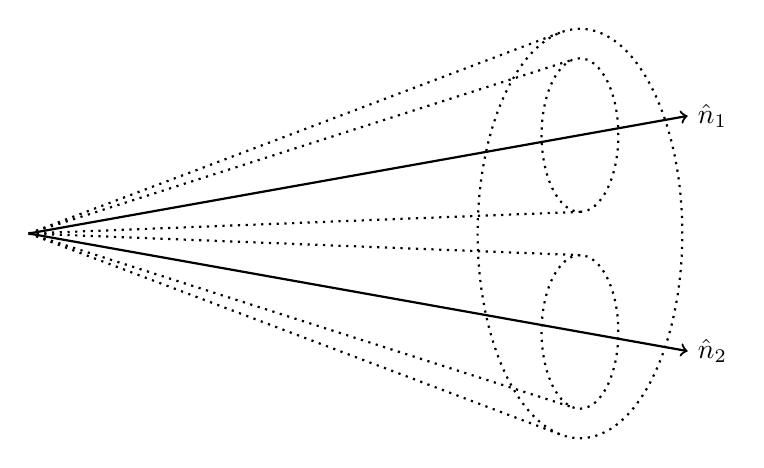
\begin{tikzpicture}
  % Main jet
  \draw[rotate around={270:(0,0)},dotted,thick] (0,7) ellipse (2.6 and 1.3);
  \draw[rotate around={270:(0,0)},dotted,thick] (0,0) -- (69.29:7.21);
  \draw[rotate around={270:(0,0)},dotted,thick] (0,0) -- (110.71:7.21);

  % Subjets
  \draw[rotate around={270:(0,0)},dotted,thick] (1.25,7) ellipse (0.975 and 0.4875);
  \draw[rotate around={270:(0,0)},dotted,thick] (0,0) -- (72.275:7.26);
  \draw[rotate around={270:(0,0)},dotted,thick] (0,0) -- (87.75:7.01);
  \draw[rotate around={270:(0,0)},dotted,thick] (-1.25,7) ellipse (0.975 and 0.4875);
  \draw[rotate around={270:(0,0)},dotted,thick] (0,0) -- (92.25:7.01);
  \draw[rotate around={270:(0,0)},dotted,thick] (0,0) -- (107.725:7.26);

  % Axes
  \draw[->,thick] (0,0) -- (10.12:8.5) node[right] {$\hat{n}_1$};
  \draw[->,thick] (0,0) -- (-10.12:8.5) node[right] {$\hat{n}_2$};
\end{tikzpicture}

%  \caption{
%    Illustration of jet substructure for a two-pronged jet with axes $\mathbf{\hat{n}}_1$ and $\mathbf{\hat{n}}_2$.
%  }
%  \label{fig:jet}
%\end{figure}

\subsection{Missing Transverse Energy}

\subsection{VBF Forward Jets}

\subsection{Spin Polarization and Boson Rapidities}

\subsection{Event Categorization}

\section{Background Modeling}
\label{sec:bkg}

%\begin{figure}[htbp]
%  \centering
%  % !TEX root = ../../thesis.tex

\begin{tikzpicture}
  \begin{feynman}
    % Vertices
    \coordinate (q1) at (135:2.25);
    \coordinate (q2) at (0,0);
    \coordinate (q3) at (225:2.25);
    \coordinate (l1) at ($(q3)+(5,0)$);
    \coordinate (l2) at ($(l1)+(-25:-1.5)$);
    \coordinate (l3) at ($(l2)+(25:1.5)$);
    \coordinate (g1) at (135:0.5625);
    \coordinate (q4) at ($(q1)+(5,0)$);
    \coordinate (q5) at ($(q4)+(25:-1.5)$);
    \coordinate (q6) at ($(q5)+(-25:1.5)$);

    \coordinate (g2) at ($(7,0)+(135:1.5)$);
    \coordinate (g3) at (7,0);
    \coordinate (g4) at ($(7,0)+(225:1.5)$);
    \coordinate (q7) at (8.5,0);
    \coordinate (q8) at ($(q7)+(55:1.5)$);
    \coordinate (q9) at ($(q7)+(-55:1.5)$);
    \coordinate (q10) at ($(q8)+(-15:1.5)$);
    \coordinate (l4) at ($(q9)+(15:1.5)$);
    \coordinate (q11) at ($(q8)+(15:1.5)$);
    \coordinate (q12) at ($(q9)+(-15:1.5)$);
    \coordinate (q13) at ($(q10)+(15:1.5)$);
    \coordinate (q14) at ($(q10)+(-15:1.5)$);
    \coordinate (l5) at ($(l4)+(15:1.5)$);
    \coordinate (l6) at ($(l4)+(-15:1.5)$);

    % Lines
    \draw[fermion] (q1) -- (q2);
    \draw[fermion] (q2) -- (q3);
    \draw[gluon] (g1) -- (q5) node[pos=0.5,above] {$g$};
    \draw[boson] (q2) -- (l2) node[pos=0.5,below] {$W$};
    \draw[fermion] (q5) -- (q4);
    \draw[fermion] (q6) -- (q5);
    \draw[fermion] (l2) -- (l1);
    \draw[fermion] (l3) -- (l2);

    \draw[gluon] (g2) -- (g3);
    \draw[gluon] (g3) -- (g4);
    \draw[gluon] (g3) -- (q7) node[pos=0.5,below] {$g$};
    \draw[fermion] (q7) -- (q8) node[pos=0.5,left] {$q$};
    \draw[fermion] (q9) -- (q7) node[pos=0.5,left] {$\bar{q}$};
    \draw[boson] (q8) -- (q10) node[pos=0.5,below] {$W$};
    \draw[boson] (q9) -- (l4) node[pos=0.5,above] {$W$};
    \draw[fermion] (q8) -- (q11);
    \draw[fermion] (q12) -- (q9);
    \draw[fermion] (q10) -- (q13);
    \draw[fermion] (q14) -- (q10);
    \draw[fermion] (l4) -- (l5);
    \draw[fermion] (l6) -- (l4);

    % Labels
    \node[anchor=mid,left] at (q1) {$q$};
    \node[anchor=mid,left] at (q3) {$\bar{q}'$};
    \node[anchor=mid,right] at (q4) {$q$};
    \node[anchor=mid,right] at (q6) {$\bar{q}$};
    \node[anchor=mid,right] at (l1) {$\ell$};
    \node[anchor=mid,right] at (l3) {$\bar{\nu}$};
    \node at (0.909,2.75) {$W$+jets};

    \node[anchor=mid,left] at (g2) {$g$};
    \node[anchor=mid,left] at (g4) {$g$};
    \node[anchor=mid,right] at (q11) {$b$};
    \node[anchor=mid,right] at (q12) {$\bar{b}$};
    \node[anchor=mid,right] at (q13) {$q''$};
    \node[anchor=mid,right] at (q14) {$\bar{q}'$};
    \node[anchor=mid,right] at (l5) {$\ell$};
    \node[anchor=mid,right] at (l6) {$\bar{\nu}$};
    \node at (9.099,2.75) {$W$+$V$/$t$};
  \end{feynman}
\end{tikzpicture}

%  \caption{
%    Feynman diagrams of the two main SM sources of background to consider for the search.
%    Both cases produce a final state that is similar to the expected final state produced by the VBF signal process.
%    The most common background is the \Wjets process (left), followed by the \WVt process (right).
%  }
%  \label{fig:bkgFeynman}
%\end{figure}

\section{Signal Modeling}
\label{sec:sig}

\section{Fit Validation and Bias Testing}
\label{sec:bias}

\section{Results}
\label{sec:results}
